\documentclass{article}
\usepackage[left=3cm,right=3cm,top=2cm,bottom=2cm]{geometry} 
\usepackage[spanish]{babel}
\usepackage[doument]{ragged2e}
\usepackage{graphicx}
\usepackage{float}
\usepackage{amsmath}
\selectlanguage{spanish}
\usepackage[utf8]{inputenc}
\setlength{\parindent}{0mm}
\usepackage{listings}

\begin{document}
\lstset{numbers=left}
\lstset{
  language=C++,
  breaklines=true,
  literate={á}{{\'a}}1
        {ã}{{\~a}}1
        {é}{{\'e}}1
        {ó}{{\'o}}1
        {í}{{\'i}}1
        {ñ}{{\~n}}1
        {¡}{{!`}}1
        {¿}{{?`}}1
        {ú}{{\'u}}1
        {Í}{{\'I}}1
        {Ó}{{\'O}}1
      }
      
\title{Práctica 1}
\author{Emilio José Hoyo Medina\\ Stefan Parvanov}
\date{\today}
\maketitle



\clearpage
\section{Condiciones de ejecución}
Los ejercicios de esta práctica se han ejecutado en ordenadores con las siguientes prestaciones:
\begin{itemize}
	\item Ejercicios 1 a 4:
	Sistema Operativo: Mac OS 10.12.6 \\ \\
	CPU: Intel Core i5 @1.6GHz	\\newline
	Memoria: 8GB ddr3 @1600Mhz	\\	
	Disco duro: 128gb SSD		\\
      \item Ejercicios 5 a 8:
        Sistema Operativo: Ubuntu 17.04 \\ \\
	CPU: Intel Core i7 @2.5GHz x 4	\\
	Memoria: 15.6GB	                \\	
	Disco duro: 1 TB HDD		\\
      \end{itemize}

      
\section{Opciones de compilación}
Para todos los ejercicios se han utilizado las siguiente formato de compilación:

\begin{verbatim}
g++ <nombrefichero>.cpp -o <nombrefichero>
\end{verbatim}
Excepto para el 6, que se ha utilizado el siguiente:
\begin{verbatim}
g++ -O3 <nombrefichero>.cpp -o <nombrefichero>
\end{verbatim}
\clearpage
\section{Ejercicio 1 : Ordenación de la burbuja}
El siguiente código realiza la ordenación mediante el algoritmo de la burbuja:
\begin{lstlisting}
      void ordenar(int *v, int n) {
        for (int i=0; i<n-1; i++)
          for (int j=0; j<n-i-1; j++)
            if (v[j]>v[j+1]) {
              int aux = v[j];
              v[j] = v[j+1];
              v[j+1] = aux;
		} 
      }
\end{lstlisting}

Calcule la eficiencia teórica de este algoritmo. A continuación replique el experimento que se ha hecho antes (búsqueda lineal) con este nuevo código. Debe:
\begin{itemize}
	\item Crear un fichero ordenacion.cpp con el programa completo para realizar una ejecución del algoritmo.
	\item Crear un script ejecuciones\_ordenacion.csh en C-Shell que permite ejecutar varias veces el programa anterior y generar un fichero con los datos obtenidos.
	\item Usar gnuplot para dibujar los datos obtenidos en el apartado previo
\end{itemize}
Los datos deben contener tiempos de ejecución para tamaños del vector 100, 600, 1100, ...,30000. \\
Pruebe a dibujar superpuestas la función con la eficiencia teórica y la empírica. ¿Qué sucede? 
\clearpage


Empezamos viendo que el bucle interior se ejecuta $\frac{(n-1)(n)}{2}$ veces.
En cada iteración se ejecutan las 4 OE de la condición del if ( incremento, dos accesos a memoria y una comparación) y  en el interior del bloque if siempre se ejecutarán 7 OE. El bucle exterior se ejecuta $(n-1)$ veces y el interior se ejecuta $\frac{(n-1)(n)}{2}$ y en cada bucle exterior se ejecutan las 3OE de la condicion del bucle(decremento, comparación, incremento) más 3 OE de la inicialización del bucle interior(asignación, resta, comparacion). Idénticamente en el bucle interior se ejecutan 3 OE del propio bucle y 3 OE del cuerpo. Además añadimos las 3 OE de la inicialización del bucle exterior:

		\begin{equation}
			T(n) = 3 + (3+3)(n-1) + \frac{(3+3+7)(n-1)(n)}{2} = \frac{13n^2 -n -6}{2}
		\end{equation}

	Nos tenemos que fijar que tenemos que dividir el número de operaciones realizadas por la frecuencia del procesador para obtener la función de tiempo.
		\begin{equation}
			T(n) = \frac{13n^2 -n -6}{2*1.6*10^9} = \frac{0.4}{10^9}n^2 - \frac{0.31}{10^9}n - \frac{1.88}{10^9} 
		\end{equation}
		\begin{equation}
						T(n) \in O(n^2)
		\end{equation}

	Representamos los datos empíricos mediante gnuplot:
	\begin{figure}[H]
  		\caption{Eficiencia empírica}
  		\centering
  		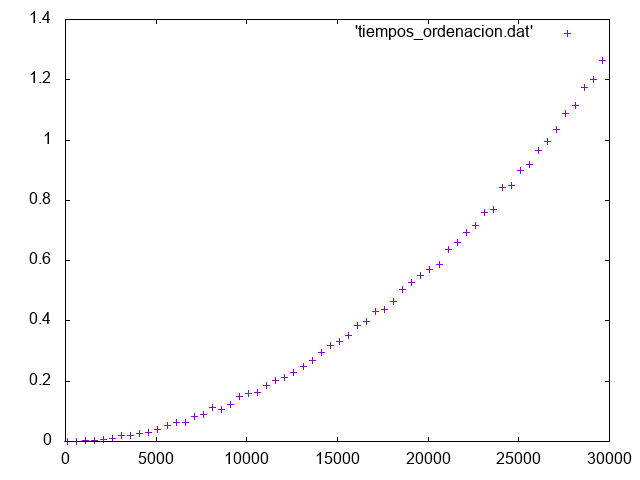
\includegraphics[width=0.8\textwidth]{ejer1/grafica.png}
	\end{figure}


\clearpage
\section{Ejercicio 2 : Ajuste en la ordenación de la burbuja}
Replique el experimento de ajuste por regresión a los resultados obtenidos en el ejercicio 1 que calculaba la eficiencia del algoritmo de ordenación de la burbuja. Para ello considere que f(x) es de la forma ax2+bx+c
\vspace{10mm}

\begin{lstlisting}
gnuplot> f(x) = a*x**2 + b*x + c
gnuplot> fit f(x) 'tiempos_ordenacion.dat' via a,b,c

.....................................................................          

After 12 iterations the fit converged.
final sum of squares of residuals : 0.00377746
rel. change during last iteration : -1.08711e-10

degrees of freedom    (FIT_NDF)                        : 57
rms of residuals      (FIT_STDFIT) = sqrt(WSSR/ndf)    : 0.00814071
variance of residuals (reduced chisquare) = WSSR/ndf   : 6.62712e-05

Final set of parameters            Asymptotic Standard Error
=======================            ==========================
a               = 1.38647e-09      +/- 1.568e-11    (1.131%)
b               = 8.02816e-07      +/- 4.812e-07    (59.94%)
c               = 0.00179818       +/- 0.003092     (171.9%)

correlation matrix of the fit parameters:
                a      b      c      
a               1.000 
b              -0.968  1.000 
c               0.738 -0.861  1.000 
\end{lstlisting}
\vspace{10mm}
	Por tanto mediante gnuplot hemos obtenido las siguiente función de ejecución:
	\begin{equation}
		T(n) = \frac{1.39x^2}{10^9} + \frac{8.03x}{10^7} + 0.0018
        \end{equation}

        Representando ahora conjuntamente los datos obtenidos y la función ajustada:
        
\begin{figure}[H]
\caption{Eficiencia empírica}
\centering
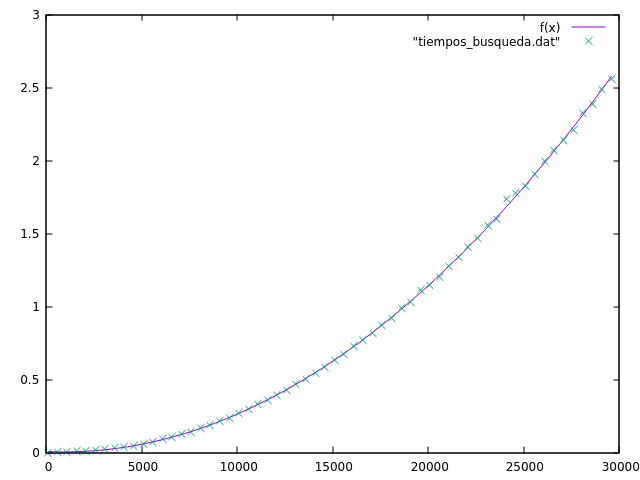
\includegraphics[width=0.8\textwidth]{ejer2/grafica.png}
\end{figure}
            

\clearpage
\section{Ejercicio 3 : Problemas de precisión}
Junto con este guión se le ha suministrado un fichero ejercicio\_desc.cpp. En él se ha implementado un algoritmo. Se pide que:
\begin{itemize}
	\item Explique qué hace este algoritmo.
	\item Calcule su eficiencia teórica.
	\item Calcule su eficiencia empírica.
\end{itemize}
Si visualiza la eficiencia empírica debería notar algo anormal. Explíquelo y proponga una solución. Compruebe que su solución es correcta. Una vez resuelto el problema realice la regresioón para ajustar la curva teórica a la empírica.\\
\clearpage


	Se trata de una búsqueda binaria. Lo que hace es buscar un valor dentro de un vector subdividiendo el vector en dos partes hasta encontrarlo. Esto solo se puede aplicar a vectores ordenados, ya que el algoritmo se basa en que si el valor no esta entre las cotas de un intervalo de valores del vector no puede estar en esas posiciones del vector. \\ \\
	Para calcular la eficiencia teórica empezamos fijandonos que el bucle principal se ejecuta $log_2(n)$ veces. Esto es asi porque podemos dividir un número entre 2 como mucho  $log_2(n)$ veces. Antes de comenzar el bucle se ejecuta 4 OE (la asignación en linea 1, las comparaciones del inicio del bucle y el AND lógico). Además dentro del bucle siempre se ejecutaran las 3 OE de la condicion y 3 OE del calculo del índice medio. Aplicando la regla de la suma en los bloques condicionales obtenemos que el máximo son 4 OE (acceso a memoria, comparación, incremento y asignación) en la segunda sentencia else if. En total en el cuerpo del bucle se ejecutaran como mucho 10 OE. Al terminar el bucle se ejecutan 2 OE más.
	En total tenemos: 
	\begin{equation}
		T(n) = 4 + (3+3+4)log_2(n) + 2 = 6+ 10log_2(n)
	\end{equation} 
	Dividimos por la frecuencia del procesador para hallar el valor en segundos:
	\begin{equation}
		T(n) = \frac{6+10log_2(n)}{1.6*10^9}
	\end{equation}
	
	Mediante gnuplot obtenemos la siguiente eficiencia empírica:
	\begin{figure}[H]
  		\caption{Eficiencia empírica}
  		\centering
  		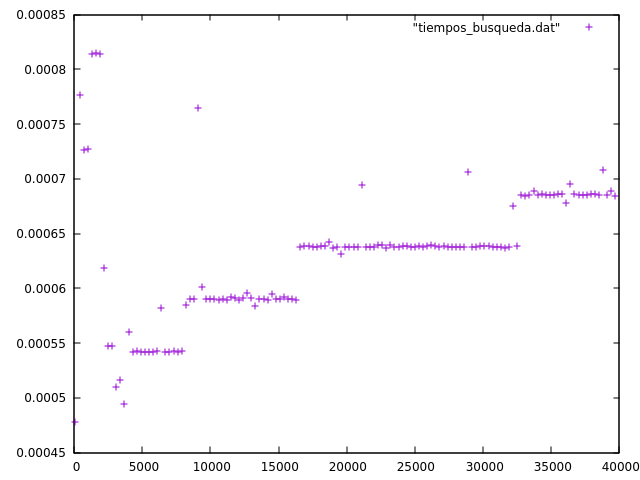
\includegraphics[width=0.8\textwidth]{ejer3/grafica.png}
	\end{figure}
	
	Como el rendimiento de la búsqueda binaria es mucho mejor que el de la ordenación de la burbuja, la ejecución para valores grandes tarda demasiado tiempo a causa de la ordenación y no podemos obtener valores fiables para trazar bien la gráfica.

\clearpage
\section{Ejercicio 4 : Mejor y peor caso}
Retome el ejercicio de ordenación mediante el algoritmo de la burbuja. Debe modificar el
código que genera los datos de entrada para situarnos en dos escenarios diferentes:
\begin{itemize}
	\item El mejor caso posible. Para este algoritmo, si la entrada es un vector que ya está ordenado el tiempo de cómputo es menor ya que no tiene que intercambiar ningún elemento
	\item El peor caso posible. Si la entrada es un vector ordenado en orden inverso estaremos en la peor situación posible ya que en cada iteración del bucle interno hay que hacer un intercambio.
\end{itemize}
	Calcule la eficiencia empírica en ambos escenarios y compárela con el resultado del ejercicio 1.
\clearpage

Sabemos que en general el tiempo que tarda el procesador en comparar dos enteros no depende de su valor y por tanto nos sirve con crear el vector de entrada más simple. Es decir, en el mejor caso el vector [0,1,2,3 ... n] y en el peor caso [n,n-1, ... ,3,2,1,0]. Además es trivial calcular la eficiencia teórica en el mejor caso, quitando las operaciones de dentro del bloque if obteniendo así:
	\begin{equation}
			T(n) = 3 + (3+3)(n-1) + \frac{(3+3+)(n-1)(n)}{2} = 3n^2 + 3n -6
	\end{equation}
Y la eficiencia teórica en el peor caso es la ya calculada en el ejercicio 1 (suponiendo que el bloque if se ejecuta siempre).
	Ejecutando la función en el mejor y peor caso obtenemos la siguiente gráfica de tiempos de ejecución de gnuplot:
		\begin{figure}[H]
  		\caption{Diferentes eficiencias}
  		\centering
  		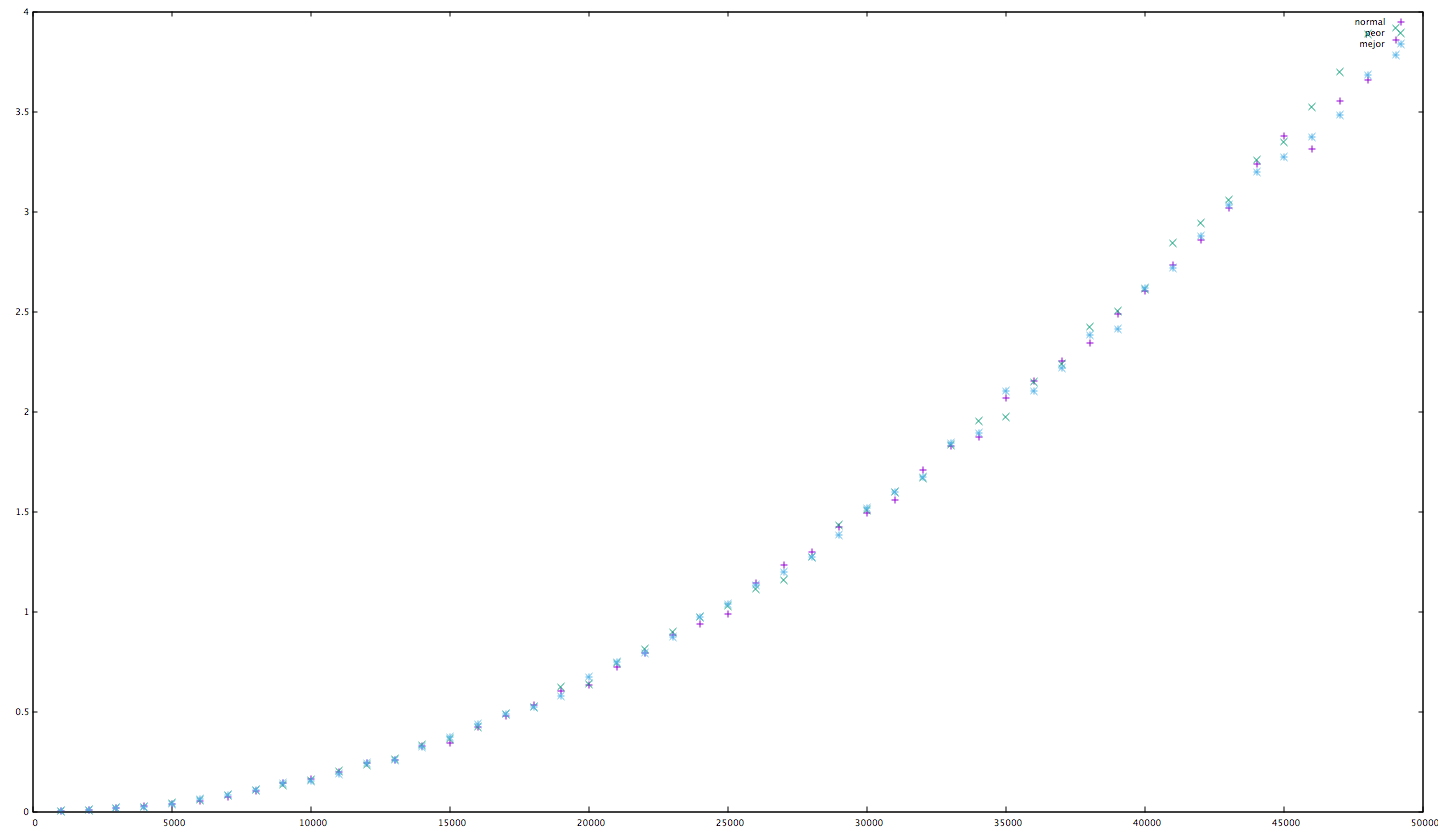
\includegraphics[width=0.8\textwidth]{ejer4/grafica.png}
	\end{figure}
	


\clearpage
\section{Ejercicio 5 : Dependencia de la implementación}
Considere esta otra implementación del algoritmo de la burbuja:
\begin{lstlisting}
	void ordenar(int *v, int n) {
		bool cambio=true;
		for (int i=0; i<n-1 && cambio; i++) {
			cambio=false;
			for (int j=0; j<n-i-1; j++)
				if (v[j]>v[j+1]) {
					cambio=true;
					int aux = v[j];
					v[j] = v[j+1];
					v[j+1] = aux;
				}
		}
	}
\end{lstlisting}

En ella se ha introducido una variable que permite saber si, en una de las iteraciones del
bucle externo no se ha modificado el vector. Si esto ocurre significa que ya está ordenado
y no hay que continuar.
Considere ahora la situación del mejor caso posible en la que el vector de entrada ya está
ordenado. ¿Cuál sería la eficiencia teórica en ese mejor caso? Muestre la gráfica con la
eficiencia empírica y compruebe si se ajusta a la previsión.
\clearpage
Empecemos calculando la eficiencia teórica:
\begin{itemize}
	\item Línea 2: 1OE (asignación).
	\item Línea 3: 1OE (asignación) + 3OE (resta, comparación,
          operación \&\&) + 1OE (incremento).
	\item Línea 4: 1OE (asignación).
	\item Línea 5: 1OE (asignación) + 3OE (resta*2, comparación) + 1OE (incremento).
	\item Línea 6: 3OE (acceso al elemento [j] y [j+1], comparación).
	\item Línea 7: 1OE (asignación).
	\item Línea 8: 2OE (acceso al elemento [j], asignación).
	\item Línea 9: 3OE (acceso al elemento [j] y [j+1], asignación).
	\item Línea 10: 2OE (acceso al elemento [j+1], asignación).
\end{itemize}
Obtenemos el siguiente tiempo de ejecución en el mejor de los casos
(con el número de línea entre paréntesis):
\begin{align*}
  T(n)= 1OE(2) + 4OE&(3) + 1OE(4) + 4OE(5) + (( 3OE(6) + 1OE(5) +
  3OE(5) )*(n-1))\\& + 1OE(3) + 3OE(3) = 14+7n-7 = 7n+7
\end{align*}
La gráfica obtenida con gnuplot es la siguiente, con tiempos de ejecución para tamaños del vector tomados de 500000 en 500000 empezando en n=1000000 y acabando en n=30000000:
\begin{figure}[H]
  \caption{Eficiencia en el mejor caso}
  \centering
  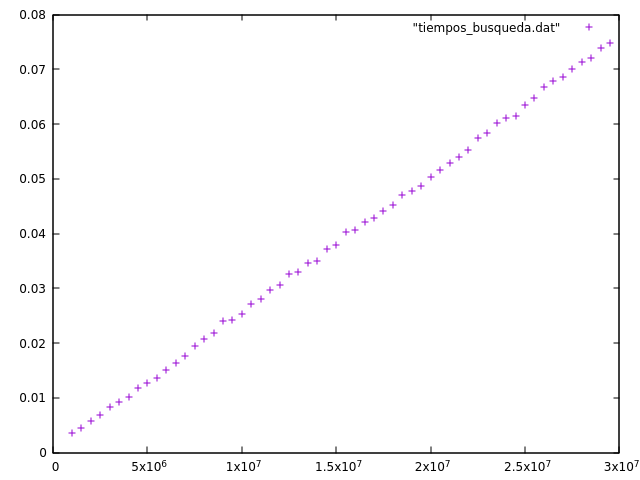
\includegraphics[width=0.8\textwidth]{ejer5/grafica.png}
\end{figure}
Como podemos ver si se ajuta a la teórica pues la mayoría de valores
de la gráfica se agrupan formando una recta.
\clearpage
\section{Ejercicio 6 : Influencia del proceso de compilación}
Retome el ejercicio de ordenación mediante el algoritmo de la burbuja. Ahora replique
dicho ejercicio pero previamente deberá compilar el programa indicándole al compilador
que optimice el código. Esto se consigue así:
\begin{verbatim}
g++ -O3 ordenacion.cpp -o ordenacion_optimizado
\end{verbatim}
Compare las curvas de eficiencia empírica para ver cómo mejora esto la eficiencia del programa.
\vspace{10mm}

La diferencia en eficiencia cuando se utiliza la opcion -O3 se puede ver claramente en la siguiente gráfica donde se han representado los datos obtenidos en ambos casos: 
\begin{figure}[H]
  \caption{}
  \centering
  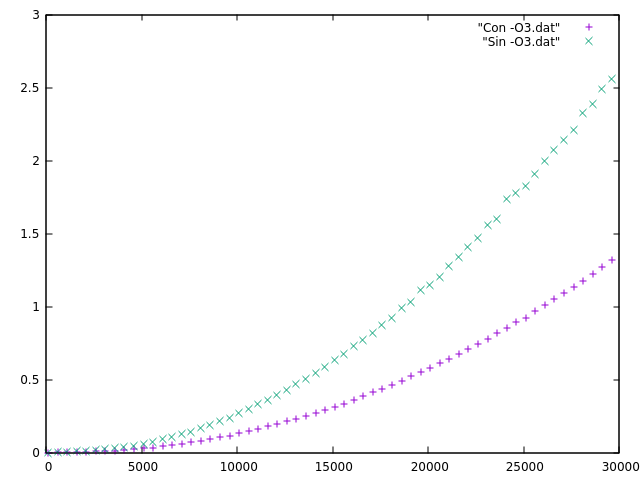
\includegraphics[width=0.8\textwidth]{comparacion.png}
\end{figure}
Se han tomado tiempos de ejecución para tamaños del vector 100, 600, 1100, ..., 30000. Podemos ver claramente como el tiempo de ejecución se reduce considerablemente.
\clearpage
\section{Ejercicio 7 : Multiplicación matricial}
Implemente un programa que realice la multiplicación de dos matrices bidimensionales.
Realice un análisis completo de la eficiencia tal y como ha hecho en ejercicios anteriores de este guión.
\clearpage

El programa a implementar quedaría tal que así:
\begin{lstlisting}
#include <iostream>
#include <ctime>    
#include <cstdlib>  

using namespace std;

void sintaxis()
{
  cerr << ``Sintaxis:'' << endl;
  cerr << ``TAM:Tamaño de la matriz (>0)'' << endl;
  cerr << ``VMAX: Valor maximo (>0)'' << endl;
  cerr << ``Se genera una matriz de tamaño TAM x TAM con elementos aleatorios en [0,VMAX['' << endl;
  exit(EXIT_FAILURE);
}

int main(int argc, char * argv[])
{
  if (argc!=3)
    sintaxis();
  int tam=atoi(argv[1]);     
  int vmax=atoi(argv[2]);    
  if (tam<=0 || vmax<=0)
    sintaxis();
  
  // Generación de la matriz aleatoria
  const int MAXIMO=800;
  int v[MAXIMO][MAXIMO],u[MAXIMO][MAXIMO], w[MAXIMO][MAXIMO];
  srand(time(0));            
  for (int i=0; i<tam; i++){
    for(int j=0;j<tam;j++){
      v[i][j]=rand() % vmax;  
      u[i][j]=rand() % vmax;
    }
  }
  int suma=0;
  clock_t tini;    
  tini=clock();
  
  for(int i=0; i<tam; i++){
    for(int j=0; j<tam; j++){
      for(int k=0; k<tam; k++){
         suma=suma+(v[i][k]*u[k][j]);
      }
      w[i][j]=suma;
      suma=0;
    }
  }

  clock_t tfin;    
  tfin=clock();

  cout << tam << "\t" << (tfin-tini)/(double)CLOCKS_PER_SEC << endl;
}
\end{lstlisting}
\clearpage
Vamos a centrarnos en el algoritmo de multiplicación de matrices:
\begin{lstlisting}
  for(int i=0; i<tam; i++){
    for(int j=0; j<tam; j++){
      for(int k=0; k<tam; k++){
         suma=suma+(v[i][k]*u[k][j]);
      }
      w[i][j]=suma;
      suma=0;
    }
  }
\end{lstlisting}
En cuanto a la eficiencia teórica, al tiempo de ejecución le corresponde la siguiente ecuación (con el número de línea al que corresponde cada conjunto de OEs entre paréntesis), donde n (=tam) es el número de filas y columnas de la matriz:
\begin{align*}
  T(n)= 2OE(1)+&2OE(2)+2OE(3)+[[[7OE(4)+2OE(3)]*n+3OE(6)+1OE(7)+\\&2OE(2)]*n+2OE(1)]*n = 9n^{3}+6n^{2}+2n+6
\end{align*}

Ahora pasamos a calcular la eficiencia empírica. Compilamos el programa y lo ejecutamos utilizando un script para n= 100, 120, 140, ..., 760, 780, 800, guardando los tiempos de ejecución obtenidos en un archivo tiempos\_matriz.dat. Obtenemos con gnuplot la siguiente gráfica:
\begin{figure}[H]
  \caption{Eficiencia en el producto de matrices nxn}
  \centering
  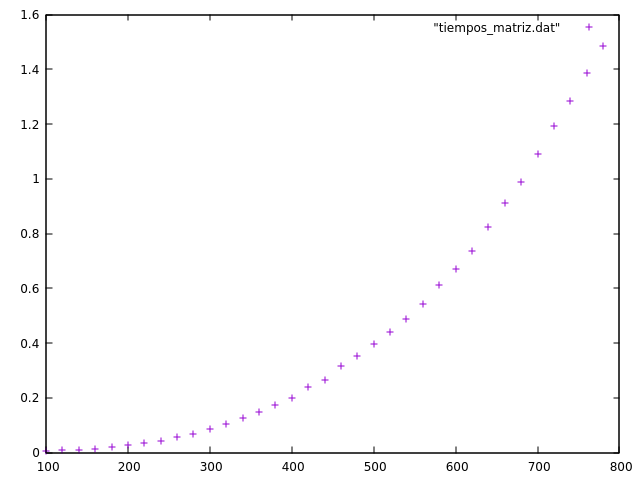
\includegraphics[width=0.8\textwidth]{graficaefic.png}
\end{figure}
Hemos de realizar un ajuste con una función de la forma:
\[
  f(x)=ax^{3}+bx^{2}+cx+d
\]
obtenemos los siguientes coeficientes usando la función fit de gnuplot:
\begin{verbatim}
Final set of parameters            Asymptotic Standard Error
=======================            ==========================
a               = 3.30848e-09      +/- 1.662e-10    (5.023%)
b               = -1.78549e-07     +/- 2.213e-07    (123.9%)
c               = 5.22417e-05      +/- 8.836e-05    (169.1%)
d               = -0.00238964      +/- 0.0102       (426.8%)

correlation matrix of the fit parameters:
                a      b      c      d      
a               1.000 
b              -0.991  1.000 
c               0.954 -0.985  1.000 
d              -0.862  0.913 -0.965  1.000 
\end{verbatim}
Ahora representamos conjuntamente f(x) y los datos obtenidos empíricamente y vemos que el ajuste es bastante bueno, es decir, la eficiencia empírica y la teórica se corresponden:
\begin{figure}[H]
  \caption{Comparación entre eficiencia empírica y teórica}
  \centering
  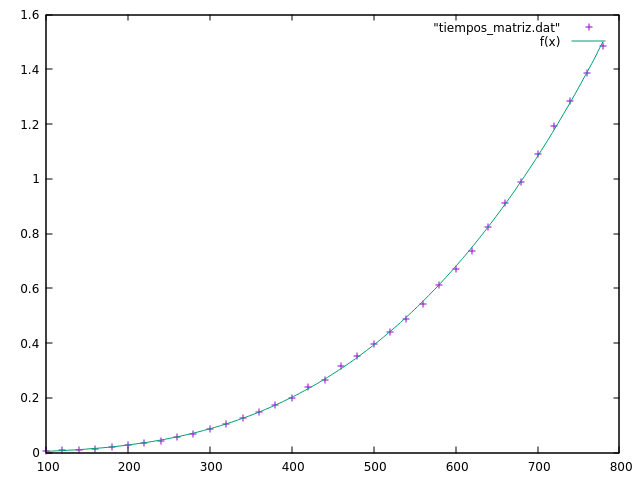
\includegraphics[width=0.8\textwidth]{graficafit.png}
\end{figure}
\clearpage
\section{Ejercicio 8 : Ordenación por Mezcla}
Estudie el código del algoritmo recursivo disponible en el fichero mergesort.cpp. En él, se integran dos algoritmos de ordenación: inserción y mezcla (o mergesort). El parámetro UMBRAL\_MS condiciona el tamaño mínimo del vector para utilizar el algoritmo de inserción en vez de seguir aplicando de forma recursiva el mergesort. Como ya habrá estudiado, la eficiencia teórica del mergesort es n log(n). Realice un análisis de la
eficiencia empírica y haga el ajuste de ambas curvas. Incluya también, para este caso, un pequeño estudio de cómo afecta el parámetro UMBRAL\_MS a la eficiencia del algoritmo. Para ello, pruebe distintos valores del mismo y analice los resultados obtenidos.
\clearpage
Para medir la eficiencia empírica compilamos el programa mergesort.cpp y lo ejecutamos mediante un script para n = 100000, 150000, 200000, ..., 3000000 guardando en un archivo tiempo\_mezcla.dat los tiempos de ejecución obtenidos. Mediante gnuplot obtenemos la siguiente gráfica:
\begin{figure}[H]
  \caption{Cálculo eficiencia empírica algoritmo de mezcla-inserción}
  \centering
  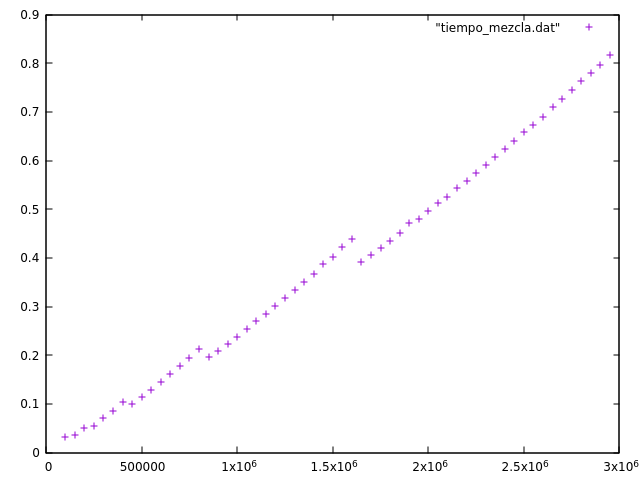
\includegraphics[width=0.8\textwidth]{mergeemp.png}
\end{figure}
Ajustamos con la función fit de gnuplot los datos con una función de la forma:
\[
  f(x) = a x log(x) + b
\]
obteniendo los siguientes valores para a y b:
\begin{verbatim}
Final set of parameters            Asymptotic Standard Error
=======================            ==========================
a               = 1.78633e-08      +/- 1.703e-10    (0.9534%)
b               = -0.000175894     +/- 0.004319     (2455%)

correlation matrix of the fit parameters:
                a      b      
a               1.000 
b              -0.867  1.000 
\end{verbatim}
\clearpage
Y obteniendose la siguiente gráfica al representar los datos empíricos y la función ajustada conjuntamente:
\begin{figure}[H]
  \caption{}
  \centering
  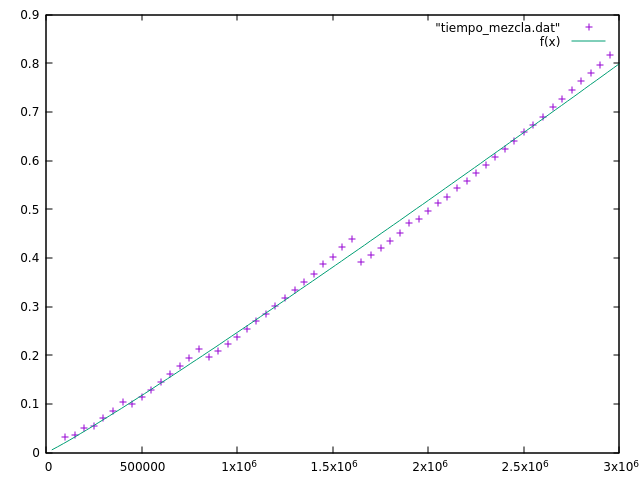
\includegraphics[width=0.8\textwidth]{mergegrafica.png}
\end{figure}
Finalmente, repetimos el cálculo de la eficiencia empírica cambiando el valor del parámetro UMBRAL\_MS. Primero lo establecemos en 200, y almacenamos los datos en un archivo tiempo\_mezcla2.dat. Luego lo establecemos en 10 y almacenamos los datos en tiempo\_mezcla3.dat. Al representar los tres conjuntos de datos obtenidos se obtiene la siguiente gráfica:
\begin{figure}[H]
  \caption{Comparación al cambiar UMBRAL\_MS}
  \centering
  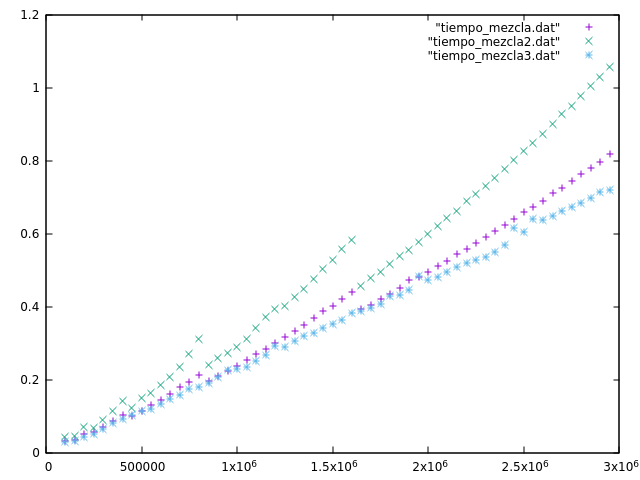
\includegraphics[width=0.8\textwidth]{mergecomp.png}
\end{figure}
Los datos de color azul corresponden al valor 10 del parámetro, y los de color verde al valor 200. El valor inicial del parámetro era 100, y por tanto podemos concluir que al aumentar el valor del parámetro UMBRAL\_MS el tiempo de ejecución aumenta y por tanto el programa es menos eficiente, y que al disminuir el valor del parámetro disminuye el tiempo de ejecución y el programa es más eficiente.
\end{document}

